\documentclass[a4paper,12pt]{article}
\usepackage[utf8]{inputenc}
\usepackage{amsmath, amssymb, amsthm, graphicx, pgfplots}
\usepackage{lmodern}
\usepackage[utf8]{inputenc}  
\usepackage[german]{babel}  
\usepackage{csquotes} 


\pgfplotsset{compat=1.18}

\title{Fourier-Methoden: Theorie und Anwendungen}
\author{Felix Wager}
\date{\today}

\begin{document}

\maketitle

\renewcommand{\contentsname}{Inhaltsverzeichnis}
\tableofcontents
\newpage

\section{Abstract}

\section{Einleitung}
\subsection{Motivation}
Warum Fourier-Methoden heute so wichtig sind.
\subsection{Zielsetzung der Arbeit}
\subsection{Aufbau der Arbeit}

\section{Mathematische Grundlagen}
\subsection{Historischer Hintergrund}
Fourier und Wärmeleitung.
\subsection{Komplexe Zahlen und die Eulerformel}
Um sich die Arbeit mit Fourier Transformationen, Reihen und sonstigem erheblich zu erleichtern ist es sehr sinnvoll mit komplexen Zahlen zu arbeiten. Doch was sind komplexe Zahlen? 
Komplexe Zahlen sind prinzipiell nichts anderes, als eine Erweiterung der Menge der Reellen Zahlen, welche es ermöglicht die Wurzel von negativen Zahlen zu ziehen. Dafür wird die Wurzel die imaginäre Einheit $i$ definiert. Mathematisch korrekt sieht das wie folgt aus:
$$i^2 = -1$$
Die Menge der komplexen Zahlen wird mit dem Symbol $\mathbb{C}$ abgekürzt. Eine typische komplexe Zahl hat in der algebraischen Schreibweise die Form:
$$ z = a + ib \quad \text{mit} \quad a,b \in \mathbb{R} $$
$a$ ist hierbei der Realteil $\Re(z)$ und $b$ der Imaginärteil $\Im(z)$ von $z$. \vspace{1em}

Um mit komplexen Zahlen bei Fourier Reihen zu arbeiten, benötigt man auch ein paar Rechenoperationen. Die wichtigsten beiden sind hier der Betrag und das komplex konjugierte einer komplexen Zahl. Eine komplexe Zahl lässt sich auch als Vektor im $\mathbb{R}^2$ betrachtet, so ist dann der Betrag als euklidische Norm dieses Vektors definiert. 
$$\vert{z}\vert = \sqrt{ a^2 + b^2}$$
Bedeutet in einem Koordinatensystem, bei dem der Real- und Imaginärteil einer Zahl auf den x- und y-Achsen festgehalten wird, ist der Betrag die Länge vom Ursprung bis zum Punkt im Koordinatensystem dieser Zahl. 
Und das komplex konjugierte einer Zahl ist eine Abbildung, welche lediglich den Imaginärteil mit $-1$ multipliziert:

$$\bar{}\;:\mathbb{C}\;\to\mathbb{C},\; z = x+iy \mapsto \bar{z} := x-iy$$

Mithilfe von komplexen Zahlen und den Taylorreihen von Sinus, Cosinus und der Exponentialfunktion $e^x$ kann man nun die Eulerformel herleiten. 

% $$e^{ix} = \cos{x} + i\sin{x}$$

Wenn man den Betrag dieses Ausdrucks bildet, so fällt auf, dass hier das Ergebnis, unabhängig von $x$, 1 ist. Dies bedeutet, dass $e^{ix}$ als ein gegen den Uhrzeigersinn rotierender Vektor, für steigende Werte für $x$, gesehen werden kann. Im vorher genannten Koordinatensystem, welches man auch die Gaußsche Zahlenebene nennt, sieht das so aus:
\begin{center}
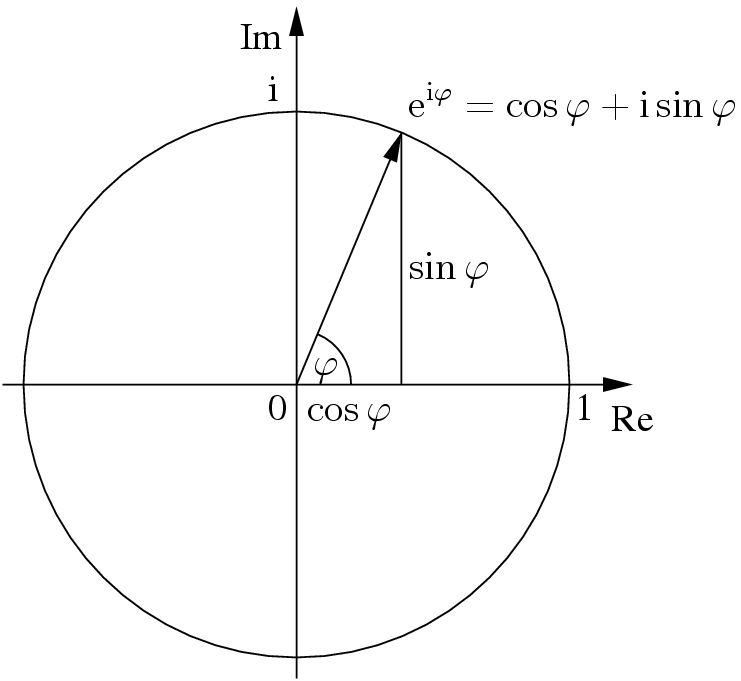
\includegraphics[scale=0.75]{eulerformel.jpg}
\end{center}

\subsection{Skalarprodukt von Funktionen und Orthonormalsysteme}
Des Weiteren spielen Orthonormalsysteme eine große Rolle, wenn man sich mit der Fourier Analyse beschäftigt. 
Allgemein lässt sich sagen, dass ein Orthonormalsystem eine Menge von Vektoren oder Funktionen, aus einem Vektorraum mit Skalarprodukt, 
sind, welche sowohl orthogonal zueinander, aber auch normiert zu sich selbst sind. 
Orthogonal sind sie, wenn das Skalarprodukt zweier unterschiedlicher Vektoren 0 ergibt und normiert, wenn das Skalarprodukt eines Vektors mit sich selbst 1 ergibt.
 Für alle Vektoren $v_n$ im $\mathbb{R}^n$ muss also folgendes gelten, damit die Menge der Vektoren ein Orthonormalsystem bildet: 
 $$\text{1. Orthogonalität: } \langle v_i, v_j\rangle = 0 \quad \forall \:i \neq j $$
 $$\text{2. Normiertheit: } \langle v_i, v_j\rangle = \sum_{i=1}^{n}v_i^2 = \|v_i\|^2 = 1 \quad \text{mit} \: i = j$$
 $$\left( \text{Skalarprodukt: } \langle v, w\rangle := \sum_{i = 1}^{n}v_i * w_i\right)$$
 Hier sieht man auch, dass das Skalarprodukt eines Vektors mit sich selbst, das gleiche 
 ist wie die quadrierte euklidische Norm des Vektors, wodurch der Begriff der Normiertheit 
 anschaulicher wird. Wie schon erwähnt lassen sich diese Eigenschaften auch auf Funktionen anwenden. 
 Hierfür definiert man die Normiertheit und die Orthogonalität auch, exakt gleich wie bei Vektoren, über das Skalarprodukt. Das Skalarprodukt für zwei Funktionen ist wie folgt definiert:
 $$\langle v, w \rangle := \int_a^bv{(x)*w(x)dx} \quad \text{für} \: v,w : [a,b] \to \mathbb{R} $$
Falls eine Menge von Funktionen Orthogonalität und Normiertheit erfüllt, ist diese Menge auch ein Orthogonalsystem. 
Anschaulich kann man sich die Funktionen v(x) und w(x) noch als zwei Vektoren mit unendlich 
vielen Dimensionen vorstellen, wobei der x Wert angibt in welcher Dimension man sich befindet. 
Da das Skalarprodukt die jeweiligen Dimensionen von Vektoren multipliziert und diese 
schließlich aufsummiert, macht es Sinn, dass man bei Funktionen ähnlich vorgeht. 
So lässt sich also die Erweiterung der Summe zum Integral erklären.  Die Formel für die 
Norm von Funktionen $\left( \|f\| = \sqrt{\int_a^b{\vert f(x)\vert^2 dx}} \right)$ ergibt sich, wenn man das für Funktionen definierte Skalarprodukt 
ähnlich wie bei Vektoren auf die Funktion selbst anwendet. Im komplexen Fall wird das Skalarprodukt leicht angepasst, 
indem der zweite Faktor komplex konjugiert wird:
$$\langle v,w \rangle := \int_a^b{v(x)*\overline{w(x)}dx} \quad \text{für} \: v,w : [a,b] \to \mathbb{C}$$


\subsection{Fourier-Reihe}
Der erste große Schritt, um die Fourier Transformation herzuleiten, ist die Fourier Reihe. 
Eine Reihe selbst ist in der Mathematik ist ein Begriff für eine unendliche Summe von Termen. 
Die Fourier Reihe ist hierbei eine besondere Reihe. Ihr Sinn ist es periodische Funktionen 
mithilfe von Sinus- und Kosinustermen zu approximieren.  Joseph Fourier hat in seinem Werk 
„Théorie analytique de la chaleur“ schließlich auch beweisen, dass jede periodische Funktion 
auf diese Weise dargestellt werden kann. Die Approximation selbst geschieht durch 
trigonometrische Polynome, mit welchen man später die Fourierreihe einer Funktion bildet. 
Ein trigonometrisches Polynom ist hier eine Funktion der Form: 
$$p(x) = a_0 + \sum_{k=1}^n{a_k \cos(kx) + b_k \sin(kx)}  \quad a_k,b_k \in \mathbb{R}$$
Ziel ist es nun die Faktoren $a_k$ und $b_k$ in Abhängigkeit zur anzunähernden Funktion zu 
bestimmen. Denn durch die Zählervariable k, welche die Periodenlänge der Sinus- und 
Kosinusterme bestimmt, kann man durch die Faktoren $a_k$ und $b_k$ festlegen wie dominant 
die Anteile der Sinus und Kosinusterme, mit der jeweiligen Periodenlänge, in der zu 
approximierende Funktion sind. Um die Berechnung der Faktoren kompakter zu gestalten, 
kann man mit dem Zusammenhang $2\cos{x} = e^{ix} -e^{-ix}$ und $2i\sin{x} = e^{ix}+e^{-ix}$, 
einer Umstellung der Eulerformel, nun das trigonometrische Polynom zu dem komplexen 
trigonometrischen Polynom zusammenfassen: 
$$p(x) = \sum_{k=-n}^n{c_k \, e^{ikx}} \quad \text{für geeignete} \: c_k \in \mathbb{C}$$
Um jetzt den komplexen Faktor $c_k$, zunächst für $2\pi$ periodische Funktionen, 
zu berechnen, verwendet man ein Orthonormalsystem, welches aus den Funktionen $\varphi_n(x)$ besteht:
$$\phi_n(x):[-\pi,\pi] \to \mathbb{C}, \quad \phi_n(x) = \frac{1}{\sqrt{2\pi}} \, e^{inx} \quad \text{mit} \: n\in \mathbb{Z}$$
Dass die Menge an Funktionen $\varphi_n$ ein Orthonormalsystem ist, habe 
ich im Anhang gezeigt (Beweis A. 1). Um endlich $c_k$ zu berechnen, setzt man zunächst 
die zu approximierende Funktion $f$, mit der Periodizität $2\pi$, mit dem 
trigonometrischen Polynom gleich und schränkt sie zudem ein: 
$$f:[-\pi,\pi]\to \mathbb{C},\quad f(x) = \sqrt{2\pi} * \sum_{k = -n}^n{c_k\phi_k(x)} $$
Anschließend bildet man das Skalarprodukt von $f$ und $\varphi_m$, was möglich ist, da 
$f$ auf der Definitionsbereich von $f$ und $\varphi_m$ gleich ist. 
$$\langle f, \phi_m \rangle = \int_{-\pi}^\pi {f(x) \overline{\phi_m(x)}dx} = \int_{-\pi}^\pi{\sqrt{2\pi}\sum_{k = -n}^n{c_k\phi_k(x)\overline{\phi_m(x)}}dx}$$
Da Integral und Summe beide linear sind, darf man die Summe mit dem Integral vertauschen. 
Zudem hängt $c_k$ nicht von $x$ ab, wodurch der Faktor $c_k$ für das Integral eine Konstante ist. 
Nach einer Abwandlung des Distributivgesetzes darf er somit herausgezogen werden. Man erhält 
also diesen Ausdruck: 
$$\int_{-\pi}^\pi{f(x)\overline{\phi_m(x)} dx} = \sqrt{2\pi}\sum_{k=-n}^{n}{c_k\int_{-\pi}^\pi{\phi_k(x) \overline{\phi_m(x)} dx}}$$
Aufgrund dessen, dass die Menge der Funktionen $\varphi_m$ ein Orthonormalsystem ist, ist jeder Summand, außer $k = m$, 0. Durch die Normiertheit des Orthonormalsystems bleibt übrig:
$$c_m = \frac{1}{\sqrt{2\pi}}\int_{-\pi}^\pi{f(x)\overline{\phi_m(x)}dx} = \frac{1}{2\pi}\int_{-\pi}^\pi{f(x)e^{imx}dx}$$ 



\section{Fourier-Reihe}
\subsection{Herleitung der Reihe}
\subsection{Berechnung der Koeffizienten}
\subsection{Eigenschaften und Konvergenz}

\section{Von der Reihe zur Fourier-Transformation}
\subsection{Übergang zum Integral}
\subsection{Fourier-Transformation und inverse Transformation}
\subsection{Eigenschaften}
Linearität, Verschiebung, Faltung.

\section{Diskrete Fourier-Transformation (DFT)}
\subsection{Definition und Motivation}
\subsection{Herleitung aus der Fourier-Transformation}
Eigene Herleitung
\subsection{Beweise für die Korrektheit}
\subsection{FFT als effiziente Berechnung}

\section{Eigene Beiträge}
\subsection{Eigene Herleitung der DFT}
\subsection{Beweise}
\subsection{Eigener FFT-Algorithmus in Python}
\subsection{Audio-Programm zur Echtzeit-Visualisierung}

\begin{figure}[h!]
\centering
\begin{tikzpicture}
\begin{axis}[
    width=\textwidth,
    height=8cm,
    xlabel={Zeit [s]},
    ylabel={Zeit [s]},
    grid=major,
    major grid style={gray!30},
    legend style={at={(0.5,-0.2)}, anchor=north, legend columns=2, font=\small},
    label style={font=\large},
    tick label style={font=\small},
    line width=1pt,
    no markers,
    cycle list={
        {blue},
        {red},
        {brown},
        {black},
        {teal}
    }
]

\addplot table[x index=1, y expr=\thisrowno{2}/1000] {fft_bench5.dat};
\addlegendentry{Rekursive FFT}

\addplot table[x index=1, y expr=\thisrowno{3}/1000] {fft_bench5.dat};
\addlegendentry{Iterative FFT}

\addplot table[x index=1, y expr=\thisrowno{4}/1000] {fft_bench5.dat};
\addlegendentry{Iterative FFT auf GPU}

\addplot table[x index=1, y expr=\thisrowno{5}/1000] {fft_bench5.dat};
\addlegendentry{cuFFT-Bibliothek (GPU)}

\addplot table[x index=1, y expr=\thisrowno{6}/1000] {fft_bench5.dat};
\addlegendentry{FFTW-Bibliothek (CPU)}


\end{axis}
\end{tikzpicture}
\caption{Vergleich der FFT-Methoden anhand der Benchmarks.}
\end{figure}

\begin{figure}[h!]
\centering
\begin{tikzpicture}
\begin{axis}[
    width=\textwidth,
    height=8cm,
    xlabel={Zeit [ms]},
    ylabel={Zeit [ms]},
    grid=major,
    major grid style={gray!30},
    legend style={at={(0.5,-0.2)}, anchor=north, legend columns=2, font=\small},
    label style={font=\large},
    tick label style={font=\small},
    line width=1pt,
    no markers,
    cycle list={
        {blue},
        {red},
        {brown},
        {black},
        {teal}
    }
]

\addplot table[x expr=\thisrowno{1}*1000, y index=2] {fft_bench_small.dat};
\addlegendentry{Rekursive FFT}

\addplot table[x expr=\thisrowno{1}*1000, y index=3] {fft_bench_small.dat};
\addlegendentry{Iterative FFT}

\addplot table[x expr=\thisrowno{1}*1000, y index=4] {fft_bench_small.dat};
\addlegendentry{Iterative FFT auf GPU}

\end{axis}
\end{tikzpicture}
\caption{Vergleich der FFT-Methoden für die zweite Messreihe.}
\end{figure}

\begin{figure}[h!]
\centering
\begin{tikzpicture}
\begin{axis}[
    width=\textwidth,
    height=8cm,
    xlabel={Zeit [min]},
    ylabel={Zeit [s]},
    grid=major,
    major grid style={gray!30},
    legend style={at={(0.5,-0.2)}, anchor=north, legend columns=2, font=\small},
    label style={font=\large},
    tick label style={font=\small},
    line width=1pt,
    no markers,
    cycle list={
        {black},
        {teal}
    }
]

\addplot table[x expr=\thisrowno{1}/60, y expr=\thisrowno{2}/1000] {fft_bench_big.dat};
\addlegendentry{cuFFT-Bibliothek (GPU)}

\addplot table[x expr=\thisrowno{1}/60, y expr=\thisrowno{3}/1000] {fft_bench_big.dat};
\addlegendentry{FFTW-Bibliothek (CPU)}

\end{axis}
\end{tikzpicture}
\caption{Vergleich der FFT-Methoden für die zweite Messreihe.}
\end{figure}

\subsection{Bildverarbeitung: Moiré-Muster entfernen mit 2D-FFT}

\section{Anwendungen}
\subsection{Audio}
Echtzeitaufnahme und Visualisierung, Tonhöhenerkennung oder Noise Cancelling, Ergebnisse.
\subsection{Bild}
Röntgenbild und Moiré-Filterung, Ergebnisse.

\section{Diskussion}
\subsection{Bewertung der Ergebnisse}
\subsection{Stärken und Grenzen}
\subsection{Bedeutung im größeren Kontext}

\section{Fazit und Ausblick}
\subsection{Zusammenfassung der Ergebnisse}
\subsection{Ausblick: Erweiterungen und Anwendungen}

\end{document}
